%===================================================================================
\section{Status of Higgs coupling fits}
%===================================================================================

\begin{figure}[b!]\centering
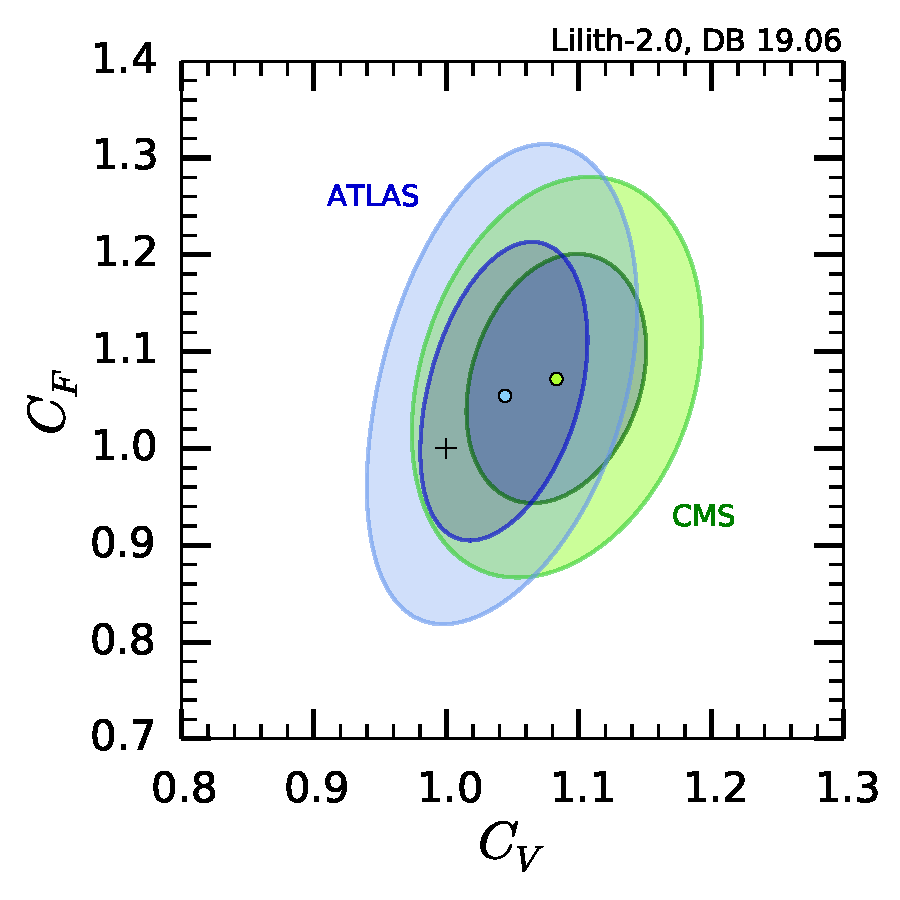
\includegraphics[width=0.5\textwidth]{fits/CVCF_2d_ATLAS_CMS.pdf}%
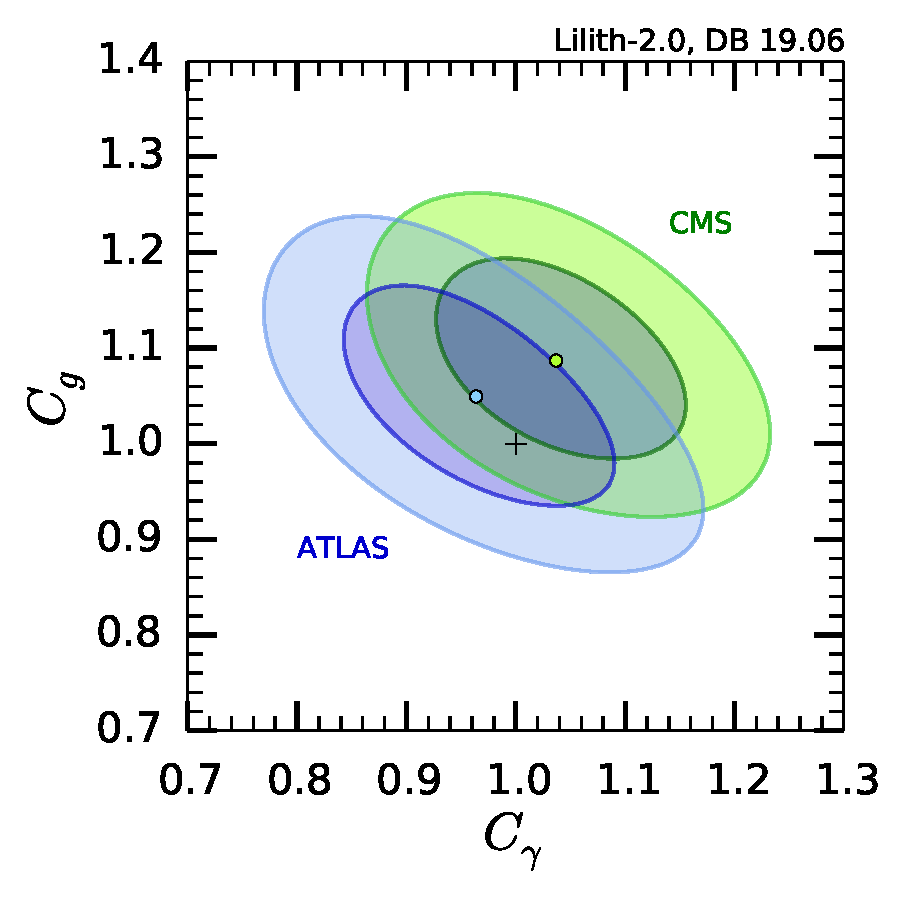
\includegraphics[width=0.5\textwidth]{fits/CgCGa_2d_ATLAS_CMS.pdf}%
\vspace*{-2mm}
\caption{Fit of $C_F$ vs.\ $C_V$ (left) and $C_g$ vs.\ $C_\gamma$ (right) using the Run~2 dataset of the 
current database version, DB~19.06. The 68\% and 95\% CL regions for the combined ATLAS results 
are shown in blue, those for CMS in green.}
\label{fig:rcfit-ATLAS-CMS}
\end{figure}

In this section we give a brief overview of the current status of Higgs coupling fits.   
We begin by showing in Fig.~\ref{fig:rcfit-ATLAS-CMS} fits of  $C_F$ vs.\ $C_V$ (left panel) and 
$C_g$ vs.\ $C_\gamma$ (right panel) using either the ATLAS (in blue) or the CMS (in green) 
Run~2 results in the current {\tt Lilith} database, DB~19.06. 
As can be seen, the two experiments agree at the level of about $1\sigma$. 

The situation when combining the results from both experiments is shown in Fig.~\ref{fig:rcfit-comb}. 
Using the Run~2 (Run~2 + Run~1) results of DB~19.06, we find   
\begin{equation}
C_F = 1.066^{+0.066}_{-0.065} ~ (1.048^{+0.056}_{-0.055}), \quad  C_V = 1.062\pm 0.030 ~ (1.059\pm 0.025) 
\end{equation}
with a correlation of $0.31$. This assumes that contributions from new particles 
to the loop-induced couplings to gluons and photons as well as invisible or undetected decays are absent. 
Taking instead $C_g$ and $C_\gamma$ as free parameters with $C_F=C_V=1$ (still assuming that 
invisible or undetected decays are absent), gives    
\begin{equation}
   C_g = 1.066^{+0.051}_{-0.050} ~ (1.070^{+0.043}_{-0.043}) , \quad  
   C_\gamma = 0.999^{+0.055}_{-0.053}~ (1.004^{+0.048}_{-0.047})
\end{equation}
with correlation $-0.52$ ($-0.51$) from Run~2 (combining Run~2 and Run~1) results.

\begin{figure}[h!]\centering
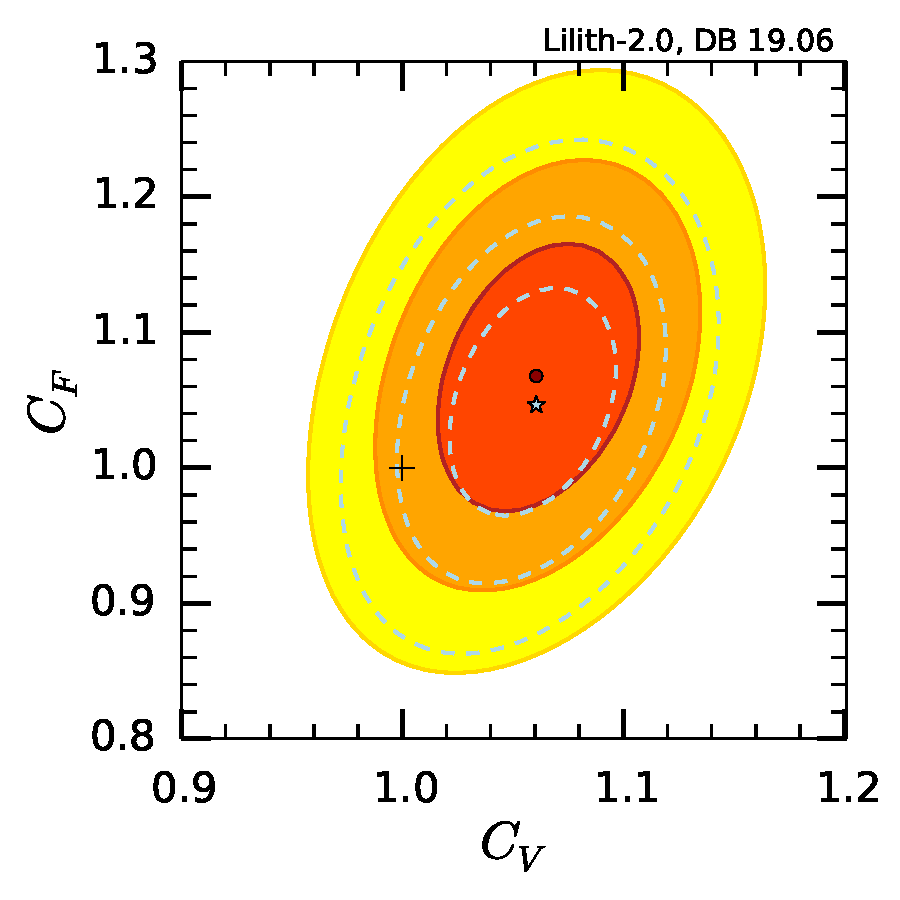
\includegraphics[width=0.5\textwidth]{fits/CVCF_2d_comb.pdf}%
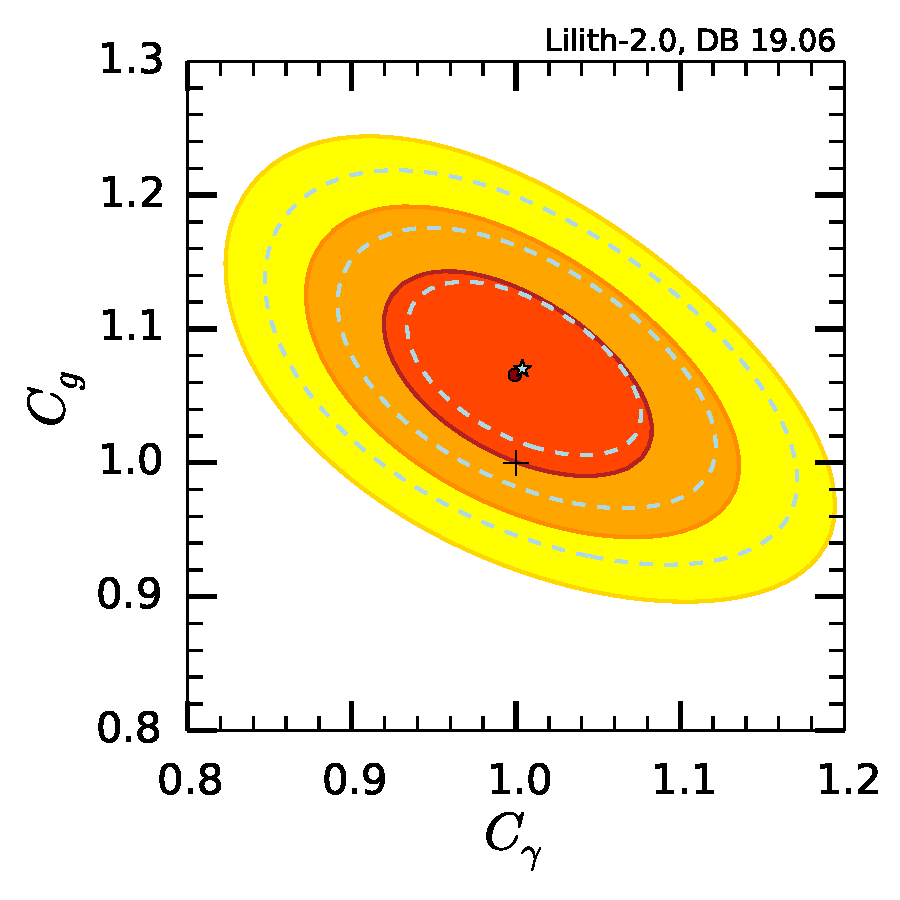
\includegraphics[width=0.5\textwidth]{fits/CgCGa_2d_comb.pdf}%
\vspace*{-2mm}
\caption{Fit of $C_F$ vs.\ $C_V$ (left) and $C_g$ vs.\ $C_\gamma$ (right) from a combination of the ATLAS and CMS 
Run~2 results in DB~19.06; the 68\%, 95\% and 99.7\% CL regions are shown as red, orange and yellow areas, respectively. 
In addition, the light-blue, dashed contours indicate the 68\%, 95\% and 99.7\% CL regions when combining the Run~2 and Run~1 data.}
\label{fig:rcfit-comb}
\end{figure}


\begin{figure}[h!]\centering
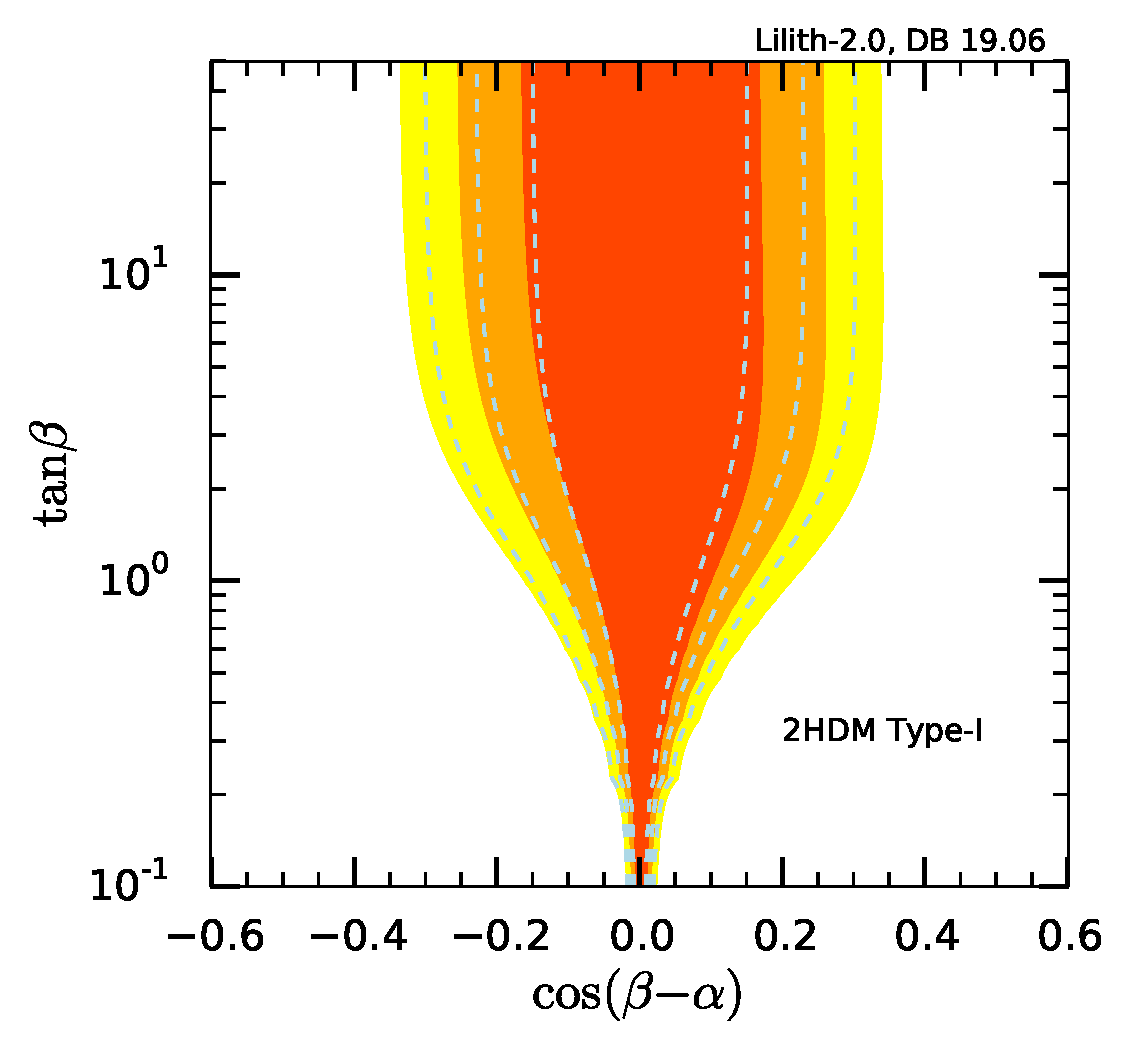
\includegraphics[width=0.5\textwidth]{fits/2HDM-type1.pdf}%
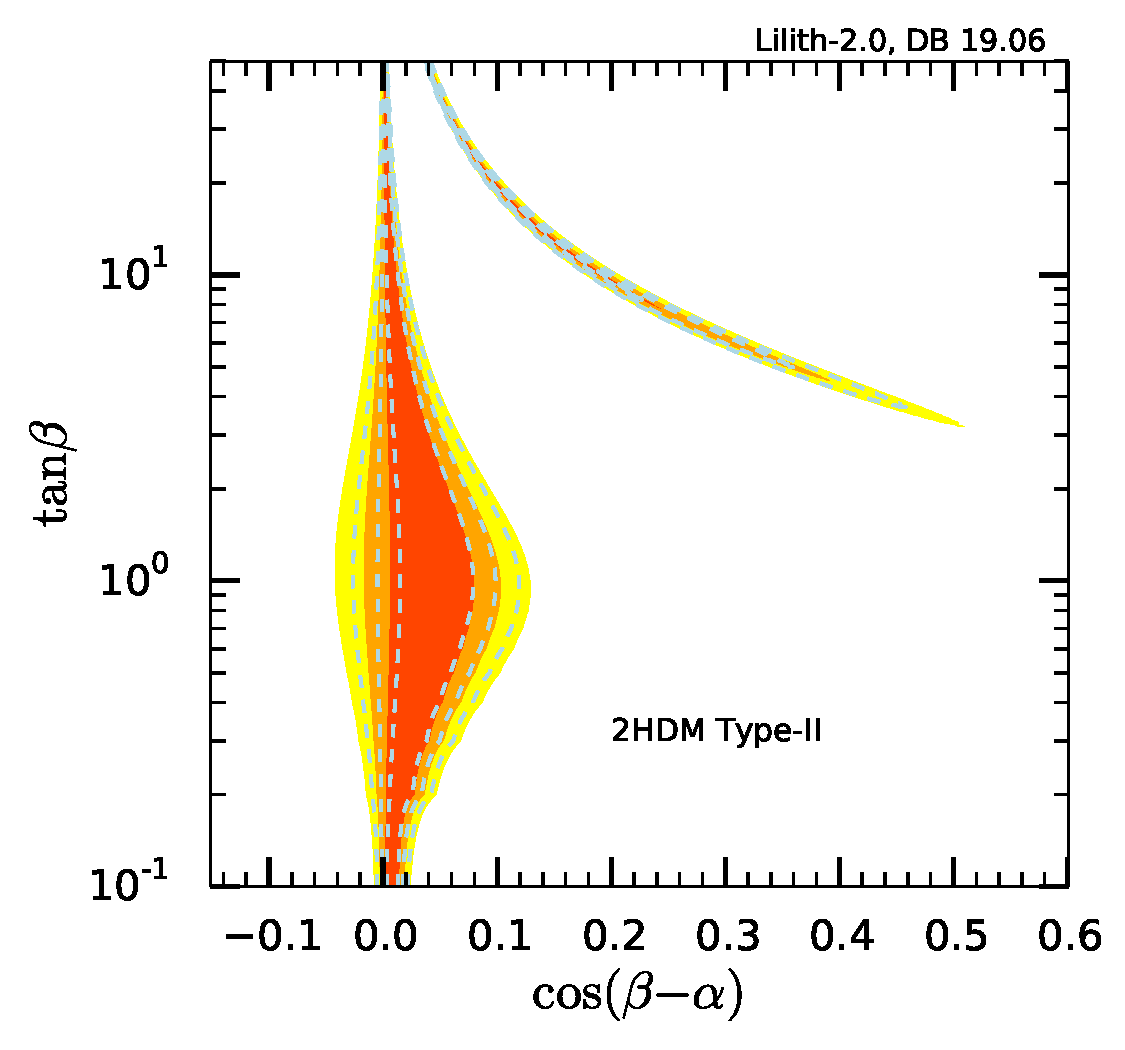
\includegraphics[width=0.5\textwidth]{fits/2HDM-type2.pdf}%
\vspace*{-2mm}
\caption{Fits of $\cos(\beta-\alpha)$ versus $\tan\beta$ for the 2HDM of Type~I (left) and of Type~II (right) 
from a combination of the ATLAS and CMS Run~2 results in DB~19.06. 
The red, orange and yellow areas are the 68.3\%, 95.4\% and 99.7\% CL regions, respectively. 
In addition, the light-blue, dashed contours indicate the 68\%, 95\% and 99.7\% CL regions when combining the Run~2 and Run~1 data. 
Loop contributions from charged Higgs bosons are neglected and decays into non-SM particles (such as $h\to AA$) assumed to be absent.}
\label{fig:2hdm-fit}
\end{figure}
